\chapter{Background \& Related Work}

In this section, constraint optimization and the distributed, as well as dynamic variants are briefly explained and brought into context of the related work. Also, the meeting scheduling problem is described and different algorithm designs and their advantages and disadvantages are explained and related work is mentioned.
    
\section{Dynamic Distributed Constraint Optimization}

% -----------------Constraint Optimization --------------------
    
A constraint optimization problem contains of a set of variables \(V=\{V_{1},V_{2}, ...,  V_{n}\}\). These variables are assigned to a value or state \(s_{j} \in S_{j}\), which is contained in a set of possible values defined by a finite problem domain \(D=\{D_{1},D_{2}, ...,  D_{n}\}\). A constraint \(C = <V_{c}, R_{c}>\) contains one (unary), two (binary) or multiple (k-ary) variables and their relationship. The constraint defines a rule for the variables that needs to be fulfilled. One of those rules could be that none of the variables should take the same value. This would for example be the case for a meeting scheduling problem where none of the meetings should take place at the same time. \newline
A utility function \(u_{{c}_{k}}(S_{{c}_{k}})\) needs to be formulated that defines a certain cost respectively reward for a given configuration of the involved states. The global utility function \(u_{g}\) would then be the summation of all utility functions of all constraints. 

\[u_{g}(s) = u_{c_{1}}(s_{c_{1}}) \oplus \cdots \oplus u_{c_{k}}(s_{c_{k}}) \oplus \cdots \oplus u_{c_{l}}(s_{c_{l}}) \] 

Constraints can be attributed with varying levels of importance through weighting. One can, instead of so-called soft constraints, define hard constraints by multiplying their utility instead of using addition in the global utility function. By defining the utility of a violated hard constraint as 0, the global utility would also go to 0 if this hard constraint is not satisfied \cite{Chapman2011, Petcu2003}. A problem only containing hard constraints would represent a constraint satisfaction problem.

\[ u_{g}(s) = \prod_{\substack{hc_{k} \in HC}} u_{SC_{g}}(s) \bigg( \sum_{sc_{k} \in SC} u_{SC_{g}}(s) \bigg)\]  % FIXME


% ----------------- Distributed Constraint Optimization --------------------
The definition of a distributed constraint problem extends the basic constraint optimization by distributing sets of variables to autonomous agents. These agents all have the goal to maximize the utility of their variables in a private utility function and thereby also contribute to a global utility function. Agents whose variables are linked to a common constraint are called neighbours \cite{Chapman2011, Farinelli, Petcu2003}.
\newline\newline 
% ----------------- Dynamic Distributed Constraint Optimization --------------------
As a further extension to the optimization, the problem definition is moved from a static to a dynamic attribute. Constraints can change and  therefore change neighbourhoods and the outcome of private and global utility functions. A change of constraints inherently changes the area of satisfying solutions if hard constraints have been included in a problem definition. Nguyen et al. state that changing the constraints might lead to the discovery of a better global optima.\cite{Nguyen2012}. Mailler et al. define a dynamic DCSP as a sequence of DCSPs \(\{P_{0}, P_{1}, ..., P_{n}\}\) where every DCSP is a static problem definition. \(P_{i}\) is therfore a result of the previous DSCP in the sequence and the added and removed constraints: \(P_{i} = P_{i-1} + c_{i^{a}} - c_{i^{r}}\) \cite{Maillera}. This definition should also hold for DCOPs. Utility functions could also be dynamically changed. Modifying this property could especially have an impact on real-world problems like meeting scheduling, where it could move the global optima from one disconnected solution space to another\cite{Nguyen2012}. Furthermore, variables could be added or removed in a dynamic setting and the problem domain \(D\) also could be changed during the course of the problem solving process.

\section{Meeting Scheduling Problem}  

%--------------------- Introduction with examples
Scheduling is the problem of allocating tasks to a given set of ressources that is usually limited with a time component. The meeting scheduling problem is a exemplary type of this family of problems. Participants of a meeting have private schedules with preferences when a meeting should be held according to their calendar. \cite{Farinelli}. 
    
One should further mention an inherent privacy aspect to the problem. Meeting participant's are often not willing to share their schedules with others except for finding a time for the specific meeting. It will later be shown that some of the algorithms can guarantee this privacy to a certain degree.
    
    %--------------------- Explanation of the components with formal definition
    
   \cite{Berger2008}
   \cite{BenHassine2007}
   \cite{Grubshtein}
   
   - hard constraints same, different
    

\section{Algorithm Design Approaches}

\begin{figure}[h]
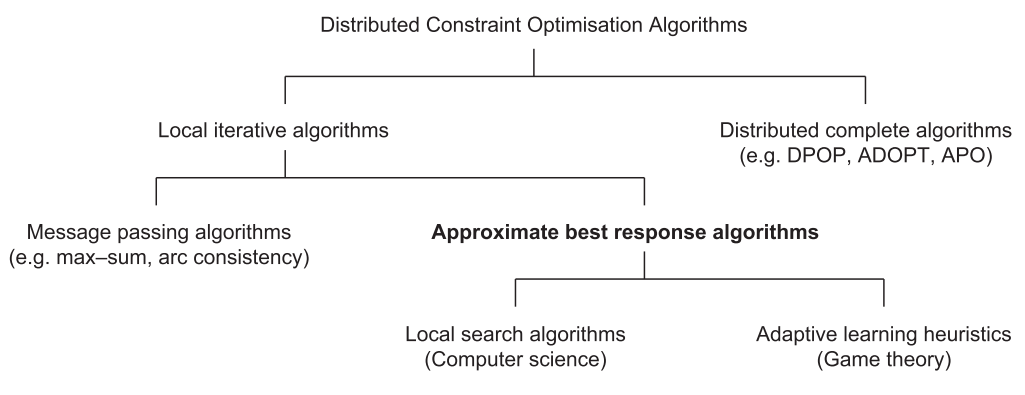
\includegraphics[width=400px]{graphics/overview_algos}
\caption{Categorization of DCO algorithms \cite{Chapman2011}}
\end{figure}

ANYTIME
SYNCHRONOUS
ASYNCHRONOUS


Distributed Constraint Optimization can be done with numerous approaches.

Other Approaches: Bee Hive optimization, Genetic Algorithms, .. DynDCOAA, SBDO, Bee Colony algorithm, Ant colony algorithm, adopt, dsa-a, dsa-b stochastic ...
    - brief related work
    - brief explanation of approaches and why they don't fit: too much information sent, centralized, too complicated, not localized
    
    The following subsections are going to explain the three chosen approaches for this thesis and which advantages, as well as disadvantages this approaches hold.
    
    \cite{Likhachev}
    
\subsection{Complete}

\cite{Chapman2011}

    - basic idea
    - advantages
    - disadvantages
    
    - dpop description

\subsection{Local-Iterative - Best Response}

- neighbourhoods
- only communicates his state
- reacts to the states of others
- privacy aspects

\cite{Chapman2011}
\cite{Maheswaran} % Achtung muss das richtig paper finden

    - Local iterative approximate best-response algorithms, such as the distributed stochastic algorithm
(Tel, 2000; Fitzpatrick  Meertens, 2003), the maximum-gain messaging algorithm (Yokoo 
Hirayama, 1996; Maheswaran et al., 2005), fictitious play (Brown, 1951; Robinson, 1951),
adaptive play (Young, 1993, 1998), and regret matching (Hart  Mas-Colell, 2000). In this class,
agents exchange messages containing only their state, or can observe the strategies of their
neighbours. In game-theoretic parlance, this is known as standard monitoring2
, and, as the name
suggests, is a typical informational assumption implicit in the literature on learning in games.


    - advantages
    - disadvantages
    
    - mgm description

\subsection{Local-Iterative - Message Passing}
    
    \cite{Chapman2011}
    - 
    
    - advantages
    -disadvantages
    - privacy aspects
    - maxsum description
    
    